\documentclass[a4paper,nofonts,nohyper,justified,colorinlistoftodos,hidelinks]{tufte-book}

\usepackage[T1]{fontenc}
\usepackage[utf8]{inputenc}
\usepackage[english]{babel}

\usepackage[a-2u]{pdfx}

\usepackage{graphicx}
\usepackage{algorithmicx}
\usepackage{algpseudocode}
\usepackage{algorithm}
\usepackage{color}
\usepackage{tikz}
\usepackage{pgfplots}
\usepackage{makeidx}
\usepackage{subfigure}
\usepackage{amssymb}
\usepackage{amsthm}
\usepackage{amsmath}
\usepackage{booktabs}
\usepackage{tensor}

\usepackage{todonotes}

\usepackage{libertine}
\usepackage{mathpazo}
\usepackage[scaled=0.83]{beramono}
\usepackage{microtype}
\usepackage{xfrac}
\usepackage{xspace}

\graphicspath{{./graphics/}}
 
%!TEX root = main.tex

%math definitions
\newcommand{\Real}{{\ensuremath{\mathbb{R}}}}
\newcommand{\Nat}{\mathbb{N}\xspace}
\newcommand{\Int}{\mathbb{Z}\xspace}
\newcommand{\Rat}{\mathbb{Q}\xspace}
\newcommand{\Prop}{\mathbb{P}\xspace}
\newcommand{\restrict}{\upharpoonright}
\newcommand{\idr}{\mathrm{Id}}
\newcommand{\normal}[2]{\mathcal{N}(#1, #2)}
\newcommand{\uniform}[2]{\mathcal{U}(#1, #2)}
\newcommand{\charf}{1}
\newcommand{\identity}{\mathrm{I}}
\newcommand{\setdiff}{\bigtriangleup}
\newcommand{\powerset}{\mathcal{P}}
\newcommand{\lequiv}{\leftrightarrow}
\newcommand{\fset}[2]{\tensor[^#1]{#2}{}}
\newcommand{\Land}{\bigwedge}
\newcommand{\Lor}{\bigvee}
\newcommand{\cons}{\theta}

\newtheorem{theorem}{Theorem}
\newtheorem{lemma}{Lemma}

\theoremstyle{definition}
\newtheorem{definition}{Definition}

\DeclareMathOperator{\Var}{var}
\DeclareMathOperator{\dom}{dom}
\DeclareMathOperator{\rng}{rng}
\DeclareMathOperator{\VF}{VF}
\DeclareMathOperator{\Thm}{Thm}
\DeclareMathOperator{\SVar}{Var}
\DeclareMathOperator{\ar}{ar}
\DeclareMathOperator{\Term}{Term}
\DeclareMathOperator{\AFm}{AFm}
\DeclareMathOperator{\Fm}{Fm}
\DeclareMathOperator{\OFm}{OFm}

\newcommand{\struct}[1]{\langle #1 \rangle}
\newcommand{\cF}{\mathcal{F}}
\newcommand{\cR}{\mathcal{R}}
\newcommand{\cA}{\mathcal{A}}

\newcommand{\twopartdef}[4]
{
	\left\{
		\begin{array}{ll}
			#1 & \text{if } #2 \\
			#3 & \text{if } #4
		\end{array}
	\right.
}
\newcommand{\twopartdefotherwise}[3]
{
	\left\{
		\begin{array}{ll}
			#1 & \text{if } #2 \\
			#3 & \text{otherwise}
		\end{array}
	\right.
}

\newcommand{\informal}[1]{\smallskip\noindent\colorbox{SkyBlue}{\begin{minipage}{\textwidth-6pt}
  \textbf{Informal! }#1
\end{minipage}}\smallskip}

% todos, comments, ...
\newcommand{\pozn}[1]{\todo[inline,color={CornflowerBlue},size=\small]{\sc{#1}}}
\newcommand{\missingref}{\todo[color={WildStrawberry}]{\textbf{Missing ref.}}}
\newcommand{\add}[1]{\todo[inline, color={YellowGreen}]{#1}}
\newcommand{\ask}[1]{\todo[inline, color={Peach}]{\textbf{???} #1}}
\newcommand{\redo}[1]{\todo[inline, color={BurntOrange}]{\textbf{<!>} #1}}

\newcommand{\code}[1]{\texttt{#1}}


% mathematical notation

\makeatletter
\renewcommand{\maketitlepage}{%
\begingroup%
\setlength{\parindent}{0pt}

%\includegraphics[width=\textwidth]{graphics/logotyp_fakulty1}

\vspace{5in}{\fontsize{36}{54}\selectfont\@title\par}
\vspace{0.5in}{\fontsize{24}{24}\selectfont\textit{\@author}\par}
\vspace{0.25in}{\fontsize{16}{16}\selectfont\textit{Based on lecture by Petr Gregor}\par}


\vfill{\fontsize{14}{14}\selectfont\textsf{\smallcaps{\@date}}\par}


\thispagestyle{empty}
\endgroup
}
\makeatother

\makeindex

\frontmatter

\title{Lecture Notes on \\ Propositional and \\ Predicate Logic}
\author{Martin Pilát}
\date{\today}

\begin{document}

\maketitle

\mainmatter

%!TEX root = main.tex

\chapter{Introduction}

Generally, logic is the study of arguments and inferences. While it started as a philosophical discipline in ancient times, it is now widely studied in mathematics and computer science. As such, logic provides the basic language and tools for most of mathematics. It studies different proof systems and discusses whether they are sound (everything they prove is valid) and complete (everything that is valid can be proven). 

While logic provides rather low-level tools for mathematics and computer science, it still has rather wide applications. For example, in some areas of artificial intelligence, logic is used to represent the knowledge of intelligent agents and reason about it. The agents then use logical reasoning (theorem proving) to decide what to do next, or prove that a certain action is safe in a given environment. Another important area is formal software verification, where logic (and, again, theorem proving) can be used to formally verify that a program indeed does what it should according to a specification. This is essential while implementing e.g. cryptographic protocols. Formal verification is also used while designing digital circuits.

There are also attempts to formalize all of mathematics in logic and use computers to check that all the proofs are correct. For example, Mizar\sidenote{\url{http://www.mizar.org/library/}} is a system that aims to re-create most of mathematics with formal and verified proofs. The verification starts from the basic mathematical axioms -- in the case of the Mizar system, authors of so called Mizar articles can use only axioms of set-theory and theorems from previously verified articles. Therefore, everything published in the Mizar mathematical library is verified to be a correct consequence of the base axioms.

Logic serves as the formal language of mathematics, and therefore logic also needs to formally specify the syntax of the language. The syntax defines what is a valid logical formula and what is not, however the meaning and validity of a formula is given by the semantics of the language. Logic itself prescribes the meaning of only a handful of symbols -- namely the logical connectives ($\land, \lor, \to, \leftrightarrow, \neg$) and the quantifiers ($\forall, \exists $). Additionally, in languages with equality, the meaning of ``$=$'' is also given. All other symbols used in logical formulas can have arbitrary meanings, which are given by the semantics. So, for example, if we write a formula $(\forall x)(\forall y)(x + y = y + x)$, we cannot discuss its validity before defining the meaning of ``$+$''. The formula is valid if we are talking about the real numbers and ``$+$'' denotes their addition.  However, the symbol ``$+$'' can also represent (quite unusually) the multiplication of square matrices, and in such a case, the formula is not valid.

There are different levels of the language of logic. In propositional logic, only propositional variables (those that are either true or false) and the logical connectives can be used. In first-order logic, we can additionally use functions, relations and quantifiers for variables that range over objects from some universe. In second-order logic, there are additionally quantifiers for sets of objects in the universe (and, more specifically, for functions and relations). In higher-order logic, we also have variables for sets of sets of objects. For example, a formula in propositional logic $$ (d \land c) \to s$$ can express that if it is dark and clear outside, the stars are visible. In a first-order language, we can have a more complex formula $$ (\forall x)(\forall y)(S(x) \land E(y) \to (L(x,y) \to P(x, y)))$$ that expresses that if $x$ is a student ($S(x)$) and $y$ is an exam ($E(y)$), if $x$ learns the material for $y$ ($L(x,y)$) then $x$ passes $y$ ($P(x,y)$). As an example of a second-order language, we can write the axiom of induction: $$ (\forall P)(P(0) \land (\forall n)(P(n) \to P(n+1)) \to (\forall n)P(n))\,.$$

In the lecture, we will deal mostly with propositional and first-order logic, however there are also other extensions of logic. For example, in multi-agent systems, so-called modal logic is often used to represent knowledge. In modal logic, there are special modalities that can further qualify a statement. For example, there is a modality that says that a statement may be true, or must be true. Other types of modal logic contain modalities that express knowledge of other agents (e.g. ``agent $A$ knows that statement $S$ is true'' can be written as $\mathrm{K}_A.S$, or even ``agent $A$ knows that agent $B$ knows that statement $S$ is true'' ($\mathrm{K}_A.\mathrm{K}_B.S$)). Another interesting type of modal logic is temporal logic, which contain modalities about time and can express e.g. ``statement $S$ will be true at some time in the future''.

\section{About these lecture notes}

In these lecture notes, logic is presented for students of computer science. Therefore, focus is given to areas most needed for computer scientists. For example, we use the more intuitive tableau method instead of Hilbert-style proof systems. We also explain the resolution method in logic as a background to Prolog and logic programming. The more advanced topics on decidability and incompleteness are explained in a more informal way.

You are currently reading the first version of the lecture notes, which can, and most probably will, contain some errors. If you find an error, or if something is not clear, do not hesitate to contact the author by e-mail\sidenote{\url{Martin.Pilat@mff.cuni.cz}}, or, alternatively, create an issue in the GitHub repository of the book\sidenote{\url{https://github.com/martinpilat/logic-book}}. 

There are also other resources you may want to check. One of them are the presentations created by Petr Gregor for his version of the lecture\sidenote{\url{http://ktiml.mff.cuni.cz/~gregor/logics/index.html}}, which serve as a base for these lecture notes.

\informal{The author of these notes sometimes likes to explain things in a more intuitive way with some not-so-formal examples and metaphors. While he  believes these can help to give a better understanding of the given concept, they sometimes (read ``often'') are rather informal and have some limitations. Therefore, in these notes, they will be set in boxes like the one you are reading just now with a bold ``\textbf{Informal!}'' warning. The information contained in these boxes is always non-essential to the rest of the text and can be (some would even argue should be) skipped.}

\section{Preliminaries}

Like many mathematical texts, these lecture notes also assume that the reader has some basic knowledge. The most important concepts (many of which should sound familiar) are briefly introduced in this short section, both to provide a single place where these can be found and to introduce the notation used in these lecture notes.

We will start with the basic set-theoretic notions. The most basic of these is the \emph{class}. Each property of sets $\varphi(x)$ defines a class $\{x|\varphi(x)\}$. Some classes are also sets; those that are not are called \emph{proper classes}. The distinction between sets and classes is probably new for most readers. Why would we need any other collections of objects than sets? How is it possible that there is a collection of objects which is not a set? The reason to distinguish between these two is that if everything were considered a set, we could find paradoxes in set theory. For example, if we had a set of all sets that do not contain themselves, does this set contain itself, or not? Let us assume, it does, but then, by definition, it does not. If we instead assume it does not contain itself, then, again, by definition, it does. This so-called Russell's paradox can be avoided by using a notion of classes that cannot contain other classes. 

\informal{A class can be understood as any collection of sets that can be described by the language of set theory. However, some of these collections do not make much sense and can lead to paradoxes. Therefore, any collection that would lead to a paradox is denoted as a proper class instead of a set and the paradoxes can thus be avoided.}

The other set-theoretic notions should be much more familiar. We use $x \in y$ to denote that $x$ is a member of set $y$. $x \notin y$ and $x \neq y$ are shortcuts for $\neg (x \in y)$ and $\neg (x = y)$. A set containing exactly elements $x_0, x_1, \dots, x_n$ is denoted as $\{x_0, x_1, \dots, x_n\}$. A set with only one element $\{x\}$ is called a \emph{singleton} and a set with two elements $\{x_0, x_1\}$ is called an \emph{unordered pair}. We will also use the common notation for set operations: $\emptyset$ denotes an \emph{empty set}, $\cup$ and $\cap$ denote the \emph{union} and \emph{intersection} of sets. $\setminus$ is the \emph{set difference} operator and $\setdiff$ is the \emph{symmetric set difference} operator $$x \setdiff y = (x \setminus y) \cup (y \setminus x)\,.$$

Two sets are \emph{disjoint} if their intersection is an empty set, and $x \subseteq y$ denotes that $x$ is a subset of $y$ (all elements of $x$ are also elements of $y$). The set of all subsets of a set $x$ -- the \emph{power set of $x$} -- is denoted as $\mathcal{P}(x)$. The \emph{union of set $x$}, $\bigcup x$, is the union of all sets contained in $x$. A \emph{cover of a set $x$} is a set $y \subseteq \mathcal{P}(x) \setminus \emptyset$ such that $\bigcup y = x$. If all the sets in the cover $y$ are mutually disjoint, then $y$ is a \emph{partition of $x$}.

The definition of an unordered pair can be used to define the \emph{ordered pair} $(a, b) = \{a, \{a,b\}\}$ and an \emph{ordered $n$-tuple} $(x_0, \dots, x_{n-1}) = ((x_0, \dots, x_{n-2}), x_{n-1})$ for $n > 2$. A Cartesian product of two sets $a$ and $b$ is $a \times b = \{(x,y) | x \in a, y \in b\}$ and the Cartesian power of a set $x$ is defined as $x^0 = \{\emptyset\}$, $x^n = x^{n-1} \times x$. A \emph{binary relation} $R$ is a set of ordered pairs. The \emph{domain of $R$} is defined as $\dom(R) = \{x|(\exists y)(x,y)\in R\}$; the \emph{range of $R$} is similarly $\rng(R) = \{y|(\exists x)(x,y)\in R\}$. The \emph{extension of $x$ in $R$} is the set $R[x] = \{y|(x,y)\in R\}$. The symbol $R^{-1}$ denotes the \emph{inverse relation} $R^{-1}=\{(y,x)|(x,y)\in R\}$. The \emph{restriction of $R$ to a set $z$} is defined as $R \restrict z = \{(x,y) \in R|x \in z\}$. Two relations can also be \emph{composed} into one, $R \circ S = \{(x,z)|(\exists y)((x,y) \in R \land (y,z) \in S\}$. The \emph{identity relation} on set $z$, $\idr_z = \{(x,x)|x\in z\}$. 

A binary function $f$ is a special type of binary relation where for every $x \in dom(f)$ there is exactly one $y$ such that $(x,y) \in f$; then $y$ is the value of $f$ in $x$ denoted as $f(x)$. $f: X \to Y$ denotes a function $f$ with $\dom(f) = X$ and $\rng(f) \subseteq Y$. The set of all such functions is $^YX$. A function $f: X \to Y$ is a \emph{surjection} (onto) if $\rng(f)=Y$, and it is an \emph{injection} (one-to-one) if for any $x,y \in dom(f)$, $x \neq y \to f(x) \neq f(y)$. A function that is both a surjection and injection is called a \emph{bijection}. Similarly to relations, we can define the inverse function $f^{-1}$, and the composition of functions $f:X\to Y$ and $g:Y\to Z$ as the function $f \circ g$ with $(f \circ g)(x) = g(f(x))$. The image of a set $A$, denoted as $f[A]$ is the set of function values for all elements of $A$, $f[A] = \{y |(x,y) \in f, x \in A\}$.

There are also two special types of relations which will be important later: equivalences and orders. An equivalence on a set $X$ is a relation that is reflexive ($R(x,x)$ for all $x\in X$), symmetric ($R(x,y) \to R(y,x)$ for $x,y \in X$) and transitive ($(R(x,y) \land R(y,z)) \to R(x,z))$ for all $x,y,z \in X$). The extension of $x$ in $R$ is called the equivalence class of $x$ and is also denoted as $[x]_R$. $X/R = \{R[x] | x \in X\}$ is the \emph{quotient set of $X$ by $R$}. The quotient set is always a partition of $X$ and every partition of $X$ also defines an equivalence on $X$ (two elements are equivalent if they are in the same set in the partition). 

The other important types of relations are the orders; usually an order is denoted as $\leq$. A relation is a \emph{partial order of a set $X$} if it is reflexive ($x \leq x$ for $x \in X$), antisymmetric ($x \leq y \land y \leq x \to x = y$ for $x,y\in X$) and transitive ($x \leq y \land y \leq z \to x \leq z$ for $x,y,z \in X$). If, additionally, for every two elements $x,y \in X$ it holds that $x \leq y$ or $y \leq x$ (dichotomy) than $\leq$ is a total (linear) order. It is a well-order if additionally every non-empty subset of $X$ has a least element. Finally, an order of $X$ is \emph{dense} if $X$ is not a singleton and for every two elements $x,y \in X$, there is another element $z \in X$ between these two ($x < y \to (\exists z) (x < z \land z < y))$, where $a < b$ means that $a \leq b \land a \neq b$. 

For example, the common ordering of natural numbers ($\leq$ on $\Nat$) is a linear well-order (as every two natural numbers are comparable and every subset of natural numbers has a least element under this order), however, it is not a dense order, as for example there is no natural number between 0 and 1. On the other hand, the common ordering of rational numbers is a dense linear order (there is a rational number between any pair of distinct rational numbers), however it is not a well-order, as e.g. the set $\{x \in \Rat\ | x \leq 0\}$ has no least element.

The natural numbers can be defined using the empty set in an inductive way -- $0 = \emptyset\,,1=\{0\} = \{\emptyset\}\,, 2=\{0,1\} = \{\emptyset, \{\emptyset\}\}\,, \dots, n=\{0, \dots, n-1\}, \dots\,.$ The set of all natural numbers $\Nat$ is the smallest set containing $\emptyset$ and closed under the operation of successor $S(x) = x \cup \{x\}$. The other common sets of numbers are the integers, which can be defined as $\Int = (\Nat \times \Nat)/\sim\,,$ with $(a,b) \sim (c,d)$ if and only if $a + d = b + c\,.$ Similarly, the set of rational numbers $\Rat$ can be defined as $\Rat = (\Int \times (\Int \setminus \{0\}))/\sim\,,$ with $(a,b) \sim (c,d)$ if and only if $ad=bc$. The definition of real numbers $\Real$ is more complex. These are usually defined as cuts of the rational numbers $\Rat$, where a cut is a partition of $\Rat$ into two sets $A$ and $B$, where all numbers in $B$ are greater than all numbers of $A$, and $A$ has no greatest element. For example, the cut corresponding to the irrational number $\sqrt{2}$ is $A = \{a\in \Rat | a^2 < 2 \lor a < 0\}\,, B = \{b\in \Rat | b^2 > 2 \land b > 0\}\,.$

Another important notion for the rest of the lecture deals with the cardinality (``size'') of sets. A set $X$ has a cardinality smaller or equal to the cardinality of a set $Y$ ($X \preceq Y$) if there is an injective function $f: X \to Y$. If there is a bijection $f: X \to Y$ then we say that $X$ and $Y$ have the same cardinality ($X \approx Y$), finally $X$ has strictly smaller cardinality than $Y$ ($X \prec Y$) if ($X \preceq Y \land \neg(X \approx Y)$). For each set $x$, there is a cardinal number $\kappa \approx x$, denoted as $|x| = \kappa$. A set $X$ is \emph{finite} if $|X| = n$ for some $n \in \Nat$. It is \emph{countable}, if it is finite or if $|x| = |\Nat| = \omega$. Otherwise, it is \emph{uncountable}. The cardinality of $\mathcal{P}(\Nat)$ is called the continuum.

It is interesting to know the cardinality of the common sets of numbers. Obviously, the set of natural numbers $\Nat$ is countable. A less obvious fact is that the sets of integers and rational numbers also have the same cardinality and are therefore also countable. For the integers, we can create an infinite sequence of integers $s = \langle 0, 1, -1, 2, -2, 3, -3, \dots \rangle$, then the function $f(i) = s_i$ is an injective function $\Nat \to \Int$, therefore $\Int \preceq \Nat$. The other inequality ($\Nat \preceq \Int$) is obvious (use identity as the injective function). In order to show that the set of rational numbers $\Rat$ is also countable, we can create a function $f(\frac{p}{q}) = 2^{|p|}3^q5^{\mathrm{sign}(p)}$ (we consider only cases where $p \in \Int, q \in \Nat \setminus \{0\}$, which clearly covers all the rationals). This is again an injective mapping $\Rat \to \Nat$ and therefore $\Rat \preceq \Nat$. As before, the other inequality is trivial. Finally, we can show that the set of real numbers $\Real$ has a larger cardinality than the set of natural numbers $\Nat$. Obviously $\Nat \preceq \Real$ as $\Nat \subseteq \Real$. Let us assume that both the sets have the same cardinality; in such a case there is a bijection $f: \Nat \to \Real$. We will now define a new real number $r$ in the following way. The integer part of the number is 0, the first digit after the decimal point is different from the first digit after decimal point in $f(0)$, the second digit is different from the second digit in $f(1)$, and so on\sidenote{If we write the decimal value of the number $r$ as $r = 0.r_0r_1r_2\dots$, where $r_i$ is the $i$-th decimal digit, we can define $r_i = (f(i)_i + 1)\, \mathrm{mod}\, 10$, where $f(i)_i$ is the $i$-th decimal digit of $f(i)$.}. This real number is different from all the numbers in $\{f(0), f(1), \dots\}$ as it differs from the number $f(i)$ in the $i$-th digit after the decimal point. This is a contradiction with the assumption that $f$ is a bijection between $\Nat$ and $\Real$ and therefore $\Nat \prec \Real$.

We will conclude our discussion of cardinalities by presenting Cantor's theorem.

\begin{theorem}[Cantor]
For every set $x$, $x \prec \powerset(x)$.
\end{theorem}

\begin{proof}
First, $f(x) = \{x\}$ is an injection $X \to \powerset(x)$ and therefore $x \preceq \powerset (x)$. Suppose there is also an injective $g: \powerset (x) \to x$. We can define a set $y = \{g(z)|z \subseteq x \land g(z) \notin z\}$. Now, similarly to Russell's paradox, $g(y) \in y$ if and only if $g(y) \notin y$, which is a contradiction, and therefore there cannot be any such injective $g$ and so $x \prec \powerset(x)$. Note that because $g$ is injective, the element $g(y)$ could belong to the set $y$ only because it fulfilled the condition (and not because it is the same as some $g(x)$ for $x \neq y$).
\end{proof}

As the tableau method used in this lecture relies on trees, we will conclude this preliminary section with a brief discussion about trees. Most of the readers are probably familiar with finite trees, however, we will sometimes need to work with infinite trees and therefore we define a \emph{tree} as a set $T$ with a partial order $<_T$ (called the tree order) with a unique least element (\emph{the root}) and in which the set of predecessors of any element is well-ordered by $<_T$. In this definition a branch is a maximal linearly ordered subset of $T$. Apart from this difference in definition, we will use the common terminology on trees from graph theory. For simplicity, we will only consider finitely branching trees, where each node except the root has an immediate predecessor\sidenote{This means, we will not deal, for example, with trees where the nodes would be set of rational numbers $\Rat$ and the tree order $<_T$ would be the common order on $\Rat$.}. In such trees we can define the \emph{levels of the tree}. The root is on level 0, the children of the nodes on the $(n-1)$-th level are on level $n$. The depth of a tree is the maximal $n \in \Nat$ of a non-empty level. In case the tree has an infinite branch it has an infinite depth $\omega$. In an $n$-ary tree, each node has at most $n$ children and a tree is finitely branching if each node has a finite number of children.

\begin{lemma}[König]
Every infinite, finitely branching tree contains an infinite branch.
\end{lemma}
\begin{proof}
The root of the tree has only finitely many children, therefore there is a child of the root that is infinite. We choose this child and continue in the same way with its children, thus constructing an infinite branch.
\end{proof}

Apart from the tree order $<_T$ we sometimes need to work with \emph{ordered trees} where the children of each node are additionally ordered from left to right with a \emph{left-to-right order} $<_L$. In a \emph{labeled tree} each node also contains an additional piece of information. For example, the formula $$(p \land q) \to q$$ can be represented as a labeled ordered tree on the right.

\begin{marginfigure}[-4\baselineskip]
\centering
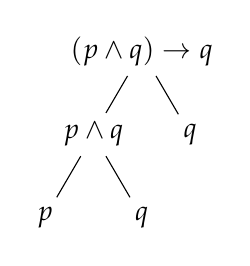
\begin{tikzpicture}[sibling distance=3.5em, level distance=3em]
  \node {$(p \land q) \to q$}
    child { node {$p \land q$} 
      child {node {$p$}}
      child {node {$q$}} }
    child { node {$q$} };
\end{tikzpicture}
\caption{The labeled ordered tree representing the formula $(p \land q) \to q$.}
\end{marginfigure}


\part{Propositional Logic}

%!TEX root = main.tex

\chapter{Propositional Formulas and Models}

In this chapter, we start the discussion of propositional logic. We will define, how propositional formulas look, what is a model in propositional logic and we will also discuss some special forms of formula.

Propositional logic is the more basic type of logic (and predicate logic is an extension of propositional logic in a sense).  Propositional formulas (propositions) are created from so called \emph{propositional variables} that represent an atomic fact which can either be true or false. These propositional variables can only be connected by common logic connectives ($\to$, $\lequiv$, $\land$, $\lor$, $\neg$). Logical formulas can additionally use parentheses to indicate priorities of connectives. While the propositional formulas are simple compared to formulas in other types of logic, they are still useful. One of the most important problems in propositional logic and in computer science in general is the satisfiability of propositional formulas (SAT). Many other NP-complete problems are often solved by transformation to the SAT problem and using one of the existing SAT solvers.

The set of propositional variables is often called $\Prop$ and the variables themselves are usually named $p, q, r, s$ or $p_0, p_1, \dots, q_0, q_1$, or similarly. Now, we can formally define the propositional formula (over $\Prop$).

\begin{definition}
Let $\Prop$ is the set of propositional variables, than
\begin{enumerate}
  \item Every propositional variable from $\Prop$ is a propositional formula.
  \item If $\varphi$ and $\psi$ are propositional formulas, than $(\varphi \to \psi), (\varphi \land \psi), (\varphi \lor \psi), (\varphi \lequiv \psi)$, and $(\neg \varphi)$ are propositional formulas.
  \item Every propositional formula is created by finite application of the two rules above.
\end{enumerate}
\end{definition}

The last part of the definition ensures that every formula is finite, this also means that each formula can contain only a finite number of distinct variables. The set of propositional variables used in a formula $\varphi$ will be denoted as $\Var(\varphi)$. On the other hand, the set of all propositional formulas using only variables from a set $\Prop$ will be denoted as $\VF_\Prop$.

Formulas are thus strings of created from propositional variables, logical connectives, and parentheses, that fulfill the conditions in the definition above. A substring of such a string that also fulfills the conditions is called a \emph{sub-formula}. 

The formal definition of formula dictates the use of parentheses around every sub-formula, which can be rather cumbersome, therefore, we define priorities of the logical connectives and can thus omit some of the parentheses. The standard priorities are such, that the negation ($\neg$) has the highest priority (therefore parentheses around $(\neg \varphi)$ can always be omitted), conjunction and disjunction ($\lor, \land$) have ``middle'' priority, and implication and equivalence ($\to, \lequiv$) have the lowest priority. Therefore, we can write $\varphi \land \psi \to \neg \varphi \lor \xi$ instead of $((\varphi \land \psi) \to ((\neg \varphi) \lor \xi))$. 

Each formula can be also represented by a so called \emph{formation tree}, which is a finite ordered tree, whose nodes are labeled with propositions -- the leaves are labeled with propositional variables, if a node has label $(\neg \varphi)$, it has a single son labeled with $\varphi$, and if a node has label $(\varphi \to \psi), (\varphi \land \psi), (\varphi \lor \psi),$ or $(\varphi \lequiv \psi)$, it has two sons, the left one has label $\varphi$, and the right one has label $\psi$. For example, a formula $p \land q \to \neg (p \lor s)$ is represented by the formation tree on the left.
\begin{marginfigure}[-4\baselineskip]
\centering
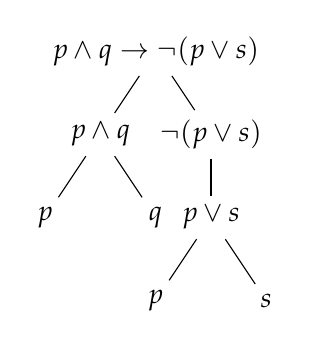
\begin{tikzpicture}[sibling distance=4em, level distance=3em]
  \node {$p \land q \to \neg (p \lor s)$}
    child { node {$p \land q$} 
      child {node {$p$}}
      child {node {$q$}} }
    child { node {$\neg (p \lor s)$}
    	child {node {$p \lor s$}
    		child {node {$p$}}
      	child {node {$s$}}}
     };
\end{tikzpicture}
\caption{The labeled ordered tree representing the formula $p \land q \to \neg (p \lor s)$.}
\end{marginfigure}

It is simple to show (by the induction on the number of nested parentheses) that each formula is associated with a unique formation tree. 

Once we have the formal definition of the formula (the syntax of propositional logic), we can define its semantics (what the formula means). The propositional variables represent atomic statements, that can have on of two truth values -- either 0 (false) or 1 (true). The truth value of the whole proposition in then given by the truth values of the variables and by the semantics of the logical connectives, which is given in Table~\ref{tab:prop_semantics} bellow.

\begin{table}[h]
\centering
\caption{The semantics of logical connectives}
\label{tab:prop_semantics}
\begin{tabular}{cc|ccccc}
\toprule
$p$ & $q$ & $\neg p$ & $p \lor q$ & $p \land q$ & $p \to q$ & $p \lequiv q$ \\
\midrule
0 & 0 & 1 & 0 & 0 & 1 & 1 \\
0 & 1 & 1 & 1 & 0 & 1 & 0 \\
1 & 0 & 0 & 1 & 0 & 0 & 0 \\
1 & 1 & 0 & 1 & 1 & 1 & 1 \\
\bottomrule
\end{tabular}
\end{table}

We can also consider the table above a definition of Boolean functions $\lor_1, \land_1, \to_1, \lequiv_1,$ and $-_1$, that implement the logical connectives. We will use these functions in cases where it is needed (e.g. while talking about truth values of propositions). More generally, any propositional formula with $n$ variables defines a Boolean function $f: \{0,1\}^n \to \{0,1\}$ (later, we will also see that any Boolean function can be expressed using a propositional formula).

We can now define the truth assignment and the truth value of formula more formally.

\begin{definition}
A \emph{truth assignment} is a function $v: \Prop \to \{0,1\}$, that is $v \in \fset{\Prop}{2}$.

A \emph{truth value} $\bar{v}(\varphi)$ of a propositional formula $\varphi$ for a truth assignment $v$ is defined inductively as:
	\begin{itemize}
		\begin{minipage}{0.5\textwidth}
		\item $\bar{v}(p) = v(p)$ if $p \in \Prop$
		\item $\bar{v}(\neg \varphi) = -_1(\bar{v}(\varphi))$ 
		\item $\bar{v}(\varphi \lor \psi) = \lor_1(\bar{v}(\varphi),\bar{v}(\psi))$ 
		\end{minipage}
		\begin{minipage}{0.5\textwidth}
		\item $\bar{v}(\varphi \land \psi) = \land_1(\bar{v}(\varphi),\bar{v}(\psi))$ 
		\item $\bar{v}(\varphi \to \psi) = \to_1(\bar{v}(\varphi),\bar{v}(\psi))$ 
		\item $\bar{v}(\varphi \lequiv \psi) = \lequiv_1(\bar{v}(\varphi),\bar{v}(\psi))$ 
		\end{minipage}
	\end{itemize}
\end{definition}

We can easily show (by the induction on the structure of the formula) that the truth value of a formula $\varphi$ depends only on the truth assignment of variables from $\Var(\varphi)$.

A proposition $\varphi$ over $\Prop$ is \emph{true in (satisfied by) an assignment} $v\in \fset{\Prop}{2}$, if $\bar{v}(\varphi) = 1$. In such a case, $v$ is called a \emph{satisfying assignment} for $\varphi$, we denote this fact $v \vDash \varphi$. If the formula is true for all assignments $v \in \fset{\Prop}{2}$, we say that it is \emph{valid (a tautology)} and denote the fact as $\vDash \varphi$. On the other hand, if there is no assignment for which the formula is true, it is called \emph{unsatisfiable (a contradiction)}. A formula $\varphi$ is \emph{independent (a contingency)} if it is neither a tautology nor a contradiction, i.e. there are two assignments $v_1, v_2 \in \fset{\Prop}{2}$, such that $\bar{v}_1(\varphi) = 1$ and $\bar{v}_2(\varphi) = 0$. Finally, a formula is \emph{satisfiable} if there is a truth assignment in it is true.

A truth assignment of $\Prop$ is also called a model of the language $\Prop$. The set of all models of $\Prop$ is denoted as $M(\Prop)$, and, obviously $M(\Prop) = \fset{\Prop}{2}$. A proposition $\varphi$ over $\Prop$ is valid in a model $v \in M(\Prop)$, if $\bar{v}(\varphi) = 1$. Then we also say that $v$ is a model of $\varphi$, denoted as $v \vDash \varphi$. $M^\Prop(\varphi) = \{v \in M(\Prop) | v \vDash \varphi\}$ is the \emph{class of all models} of $\varphi$. A formula is valid, if it is true in every model of the language, it is unsatisfiable if it does not have a model, and satisfiable if it has a model. It is independent if it is true in a model of the language and false in another one. Formulas $\varphi$ and $\psi$ are logically equivalent ($\varphi \sim \psi$, if $M^\Prop(\varphi) = M^\Prop(\psi)$.

The last two paragraphs say basically the same, the difference is that in the latter one, we use the notion of model, which is central to logic. The notion of models, and sets of models will be important later, and ``model'' is one of the key term in logic.

In the definition of propositions, we used 5 different logical connectives. However, if we take a look at the table with their semantics, we may notice, that, for example, $p \to q$ is equivalent $\neg p \lor q$. Therefore, even without using the implication ($\to$) we can still express everything we could with them. More formally, for every formula $\varphi \in \VF_\Prop$, there is an equivalent formula $\varphi'$ that does not use the implication. Moreover, we can notice, that $p \lequiv q$ is equivalent to $(p \to q) \land (q \to p)$, therefore we even do not need the equivalence, and every formula can be written using only negation, conjunction, and disjunction ($\neg, \land, \lor$). This feature of the set can be defined more formally.

\begin{definition}
A set of connectives is \emph{adequate} if they can express any Boolean function by some proposition from them.
\end{definition}

We have already discussed that the set ($\neg, \land, \lor$) is adequate. We can also show, that the set $\{\to, \neg\}$ is adequate, the easiest way to do that is to realize, that $(p \land q) \sim \neg (p \to \neg q)$ and $(p \lor q) \sim (\neg p \to q)$. 

Generally, we can also define custom connectives, for example, the so called Shaffer stroke (NAND) is defined as $p \uparrow q \sim \neg (p \land q)$, or the Pierce arrow (NOR) is defined as $p \downarrow q \sim \neg (p \lor q)$. Interestingly, both $\{\uparrow\}$ and $\{\downarrow\}$ are adequate sets. This is an important fact for the construction of logical circuits as we can use a logical gate of only one kind (either NAND or NOR) to express any Boolean function.

There are also special forms of formulas, which are often used. Among the most common ones are so called conjunctive and disjunctive normal forms. In order to define these two forms, we first need to define a literal. A \emph{literal} is a propositional variable or its negation, for example, if $\Prop = \{p, q\}$ then all the literals we can construct over $\Prop$ are $\{p, \neg p, q, \neg q\}$. A formula is in conjunctive normal form (CNF) if it is a conjunction of disjunctions of literals. Disjunctions of literals are also called \emph{clauses}, therefore we can also say, that a CNF formula is a conjunction of clauses. On the other hand, a formula is in disjunctive normal form (DNF) if it is a disjunction of conjunctions of literals. So, for example, $(p \lor \neg q \lor r) \land (p \lor q) \land (\neg p \lor q \lor r)$ is a formula in CNF and$(\neg p \land q \land \neg r) \lor (\neg p \land \neg q) \lor (p \land \neg q \land \neg r)$ is a formula in DNF (and, moreover a negation of the previous one in CNF). 

Now, we would like to show, that for every formula, there is an equivalent formula in CNF and another equivalent formula in DNF. To this end, we will need to following set of rules, which can be proved manually by checking the truth table of the propositional connectives: 

\begin{enumerate}
  \item $(\varphi \to \psi) \sim (\neg \varphi \lor \psi), (\varphi \lequiv \psi) \sim ((\neg \varphi \lor \psi) \land (\neg \psi \lor \varphi))$
  \item $\neg \neg \varphi \sim \varphi, \neg (\varphi \land \psi) \sim (\neg \varphi \lor \neg \psi), \neg (\varphi \lor \psi) \sim (\neg \varphi \land \neg \psi)$
  \item $(\varphi \lor (\psi \land \chi)) \sim ((\psi \land \chi)  \lor \varphi) \sim ((\varphi \lor \psi) \land (\varphi \lor \chi))$
  \item $(\varphi \land (\psi \lor \chi)) \sim ((\psi \lor \chi)  \land \varphi) \sim ((\varphi \land \psi) \lor (\varphi \land \chi))$
\end{enumerate}

We can also easily show (again by induction on the structure of the formula) that if we have a formula $\varphi'$ which is obtained from $\varphi$ by replacing some occurrences of its sub-formula $\psi$ with an equivalent sub-formula $\psi'$, then $\varphi \sim \varphi'$.

And finally, we can show the following theorem. 

\begin{theorem}
For every formula $\varphi$ over $\Prop$, there are formulas $\varphi_C$ and $\varphi_D$, such that $\varphi_C$ is in CNF, $\varphi_D$ is in DNF and $\varphi \sim \varphi_C$ and $\varphi \sim \varphi_D$.
\end{theorem}
\begin{proof}
The propositions $\varphi_C$ and $\varphi_D$ can be obtained from $\varphi$ by applying the rules 1 to 4 mentioned above. 
\end{proof}

The discussion above shows one of the ways to obtain equivalent formulas in CNF and DNF to a given formula. We can in fact apply the rules in the order, in which they are presented. First, we remove all the implications and equivalences by using the rules no. 1. Then, we move all negations to the literals (i.e. there are no negations outside of parentheses), using the rule no. 2 and, finally, we repeatedly apply rules no. 3 and 4 to obtain the CNF and DNF. 

This syntactic approach is not the only one to obtain CNF/DNF from a given formula. We can also construct the truth table of the formula and then read the CNF/DNF almost directly from the table. We will show a more general approach here, we will construct a CNF and DNF formulas $\varphi_C$ and $\varphi_D$ such that $M^\Prop(\varphi_C) = M^\Prop(\varphi_D) = K \subseteq M(\Prop)$, for a given finite set of truth assignments $K$. 

Before we show the construction, we will define the notion of $p^t$ for a variable $p$ and a truth value $t$ as $$ p^t \twopartdef{p}{t = 1}{\neg p}{t = 0}\,.$$ 

Now, we can easily see that for a single assignment $v \in K$, the set of models of the formula $\Land_{p \in \Prop} p^{v(p)}$ contains only $v$. For a set of assignments $K$, we can just make a disjunction over all assignments in $K$ (remember $K$ is a finite set). Therefore, $$M(\Lor_{v \in K}\Land_{p \in \Prop}p^{v(p)}) = K\,.$$ Thus we constructed a formula in DNF whose models are exactly the set $K$. 

Constructing a formula $\varphi$ in CNF such that $M(\varphi) = K$ for some given finite $K$ is slightly more complex. However, we can use the fact that the negation of a formula in DNF is a formula in DNF. Negating a formula in CNF means changing all the conjunctions to disjunctions and vice versa and changing all literals to the complementary ones (i.e. changing $p$ to $\neg p$ and vice versa). So, we start by creating a formula $\neg \varphi$ in DNF for the set $\fset{\Prop}{2} \setminus K$ according to the approach above. Then, we negate the formula, thus obtaining $\varphi$ in CNF such that $M(\varphi)=K$. Following these two steps we obtain the formula $$\varphi = \Land_{v \in \fset{\Prop}{2} \setminus K}\Lor p^{-_1v(p)}$$ such that $M(\varphi) = K$.

If we want to use this approach to create a formula in CNF or DNF equivalent to a formula $\varphi$, we simply choose $K=M(\varphi)$. This description also shows that any Boolean function $f$ (i.e. function $f: \{0,1\}^n \to \{0,1\}$) can be expressed as a proposition. We can choose $K = \{v | f(v) = 1\}$. 

Both the techniques described above lead to an equivalent formula in CNF/DNF. Choosing the better one for the task depends on a few features of the ``input'' formula. Typically, the table-based method is preferred for formulas with only a few variables (as the size of the table grows exponentially with the number of variables). 


\backmatter

\setcounter{tocdepth}{2}
\tableofcontents
\listoffigures
\listoftables
\listofalgorithms 
\listoftodos

\end{document}
